% -----------------------------------------------------------------------------
%						A History
% -----------------------------------------------------------------------------
\section{History}
\label{sect:history}

% A.1 Acknowledgments
% -------------------------------------------------------------
\subsection{Acknowledgments}
\label{sect:acks}

\begin{itemize}
	\item
    The first 6 to 6.5 versions of this manual and early UGE job script samples, Singularity testing,and user support
    were produced/done by Dr.~Scott Bunnell during his time at Concordia as a part of the NAG/HPC group.
    We thank him for his contributions.
	\item
    The HTML version with devcontainer support was contributed by Anh H Nguyen.
	\item
    Dr.~Tariq Daradkeh, was our IT Instructional Specialist from August 2022 to September 2023;
    working on the scheduler, scheduling research, end user support, and integration of
    examples, such as YOLOv3 in \xs{sect:openiss-yolov3} and other tasks. We have a continued
    collaboration on HPC/scheduling research (see~\cite{job-failure-prediction-compsysarch2024}).
\end{itemize}

% A.2 Migration from UGE to SLURM
% -------------------------------------------------------------
\subsection{Migration from UGE to SLURM}
\label{appdx:uge-to-slurm}

For long term users who started off with Grid Engine here are some resources
to make a transition and mapping to the job submission process.

\begin{itemize}
\item
Queues are called ``partitions'' in SLURM. Our mapping from the GE queues to SLURM partitions is as follows:
\begin{verbatim}
    GE  => SLURM
    s.q    ps
    g.q    pg
    a.q    pa
\end{verbatim}
We also have a new partition \texttt{pt} that covers SPEED2 nodes, which previously did not exist.

\item
Commands and command options mappings are found in \xf{fig:rosetta-mappings} from:\\
\url{https://slurm.schedmd.com/rosetta.pdf}\\
\url{https://slurm.schedmd.com/pdfs/summary.pdf}\\
Other related helpful resources from similar organizations who either used SLURM for a while or also transitioned to it:\\
\url{https://docs.alliancecan.ca/wiki/Running_jobs}\\
\url{https://www.depts.ttu.edu/hpcc/userguides/general_guides/Conversion_Table_1.pdf}\\
\url{https://docs.mpcdf.mpg.de/doc/computing/clusters/aux/migration-from-sge-to-slurm}

\begin{figure}[htpb]
    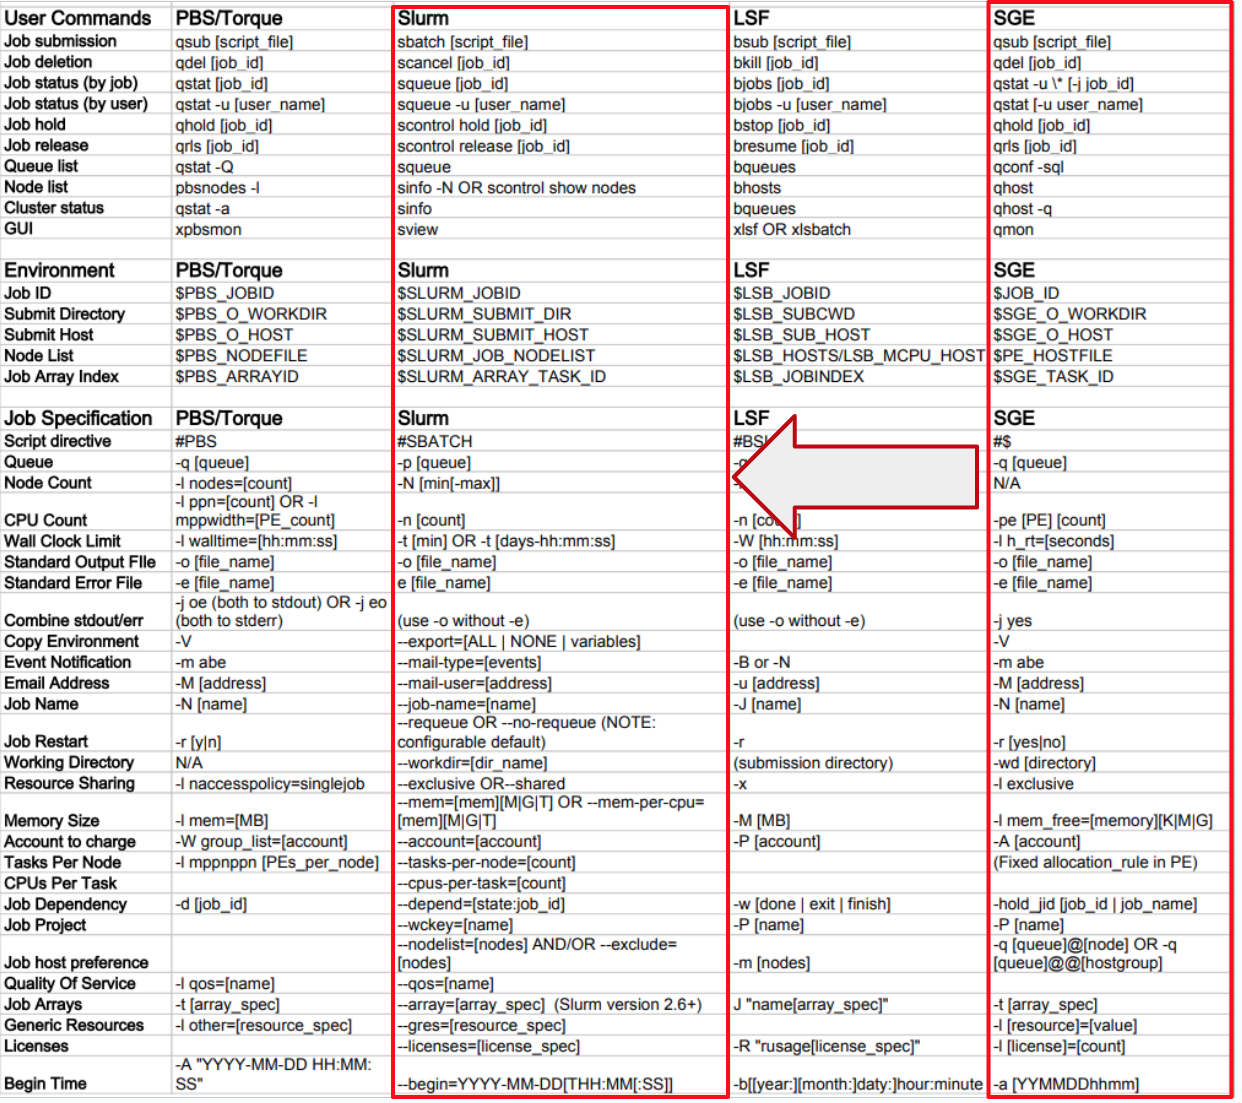
\includegraphics[width=\columnwidth]{images/rosetta-mapping}
    \caption{Rosetta Mappings of Scheduler Commands from SchedMD}
    \label{fig:rosetta-mappings}
\end{figure}

\item
\textbf{NOTE:} If you have used UGE commands in the past you probably still have these
lines there; \textbf{they should now be removed}, as they have no use in SLURM and
will start giving ``command not found'' errors on login when the software is removed:

csh/\tool{tcsh}: sample \file{.tcshrc} file:
\scriptsize
\begin{verbatim}
    # Speed environment set up
    if ($HOSTNAME == speed-submit.encs.concordia.ca) then
    source /local/pkg/uge-8.6.3/root/default/common/settings.csh
    endif
\end{verbatim}
\normalsize
Bourne shell/\tool{bash}: sample \file{.bashrc} file:
\scriptsize
\begin{verbatim}
    # Speed environment set up
    if [ $HOSTNAME = "speed-submit.encs.concordia.ca" ]; then
        . /local/pkg/uge-8.6.3/root/default/common/settings.sh
        printenv ORGANIZATION | grep -qw ENCS || . /encs/Share/bash/profile
    fi
\end{verbatim}
\normalsize

\textbf{IMPORTANT NOTE:} you will need to either log out and back in, or execute a new shell, 
for the environment changes in the updated \file{.tcshrc} or \file{.bashrc} file to be applied.
\end{itemize}

% A.3 Phases
% -------------------------------------------------------------
\subsection{Phases}
\label{sect:phases}

Brief summary of Speed evolution phases:

\subsubsection{Phase 6}
Phase 6 had 2 new nodes (cisr) from doctor Suryadipta Majumdar.

\subsubsection{Phase 5}
Phase 5 saw incorporation of the Salus, Magic, and Nebular
subclusters (see \xf{fig:speed-architecture}).

\subsubsection{Phase 4}
Phase 4 had 7 SuperMicro servers with 4x A100 80GB GPUs each added,
dubbed as ``SPEED2''. We also moved from Grid Engine to SLURM.

\subsubsection{Phase 3}
Phase 3 had 4 vidpro nodes added from Dr.~Amer totalling 6x P6 and 6x V100
GPUs added.

\subsubsection{Phase 2}
Phase 2 saw 6x NVIDIA Tesla P6 added and 8x more compute nodes.
The P6s replaced 4x of FirePro S7150.

\subsubsection{Phase 1}
Phase 1 of Speed was of the following configuration:
\begin{itemize}
    \item
    Sixteen, 32-core nodes, each with 512~GB of memory and approximately 1~TB of volatile-scratch disk space.
    \item
    Five AMD FirePro S7150 GPUs, with 8~GB of memory (compatible with the Direct X, OpenGL, OpenCL, and Vulkan APIs).
\end{itemize}